\documentclass[fleqn]{article}
\oddsidemargin 0.0in
\textwidth 6.0in
\thispagestyle{empty}
\usepackage{import}
\usepackage{amsmath}
\usepackage{graphicx}
\usepackage{flexisym}
\usepackage{calligra}
\usepackage{amssymb}
\usepackage{bigints} 
\usepackage[english]{babel}
\usepackage[utf8x]{inputenc}
\usepackage{float}
\usepackage[colorinlistoftodos]{todonotes}


\DeclareMathAlphabet{\mathcalligra}{T1}{calligra}{m}{n}
\DeclareFontShape{T1}{calligra}{m}{n}{<->s*[2.2]callig15}{}
\newcommand{\scriptr}{\mathcalligra{r}\,}
\newcommand{\boldscriptr}{\pmb{\mathcalligra{r}}\,}

\definecolor{hwColor}{HTML}{442020}

\begin{document}

  \begin{titlepage}

    \newcommand{\HRule}{\rule{\linewidth}{0.5mm}}

    \center

    \begin{center}
      
\includegraphics[height=11cm, width=11cm]{asu.png}
    \end{center}

    \vline

    \textsc{\LARGE Statistical/Thermal Physics}\\[1.5cm]

    \HRule \\[0.5cm]
    { \huge \bfseries Quiz 7}\\[0.4cm] 
    \HRule \\[1.0cm]

    \textbf{Behnam Amiri}

    \bigbreak

    \textbf{Prof: Michael Treacy}

    \bigbreak

    \textbf{{\large \today}\\[2cm]}

    \vfill

  \end{titlepage}

  By signing my name, I am promising that I did this quiz on my own without any outside help.

  \vspace{0.5cm}

  Name: \textbf{Behnam Amiri}

  \vspace{1cm}



  \begin{enumerate}
    \item An ethanol $(C_2 H_5 OH)$ fuel cell uses the spontaneous redox reaction
    $$
      C_2 H_5 OH+3O_2 \longrightarrow 3 H_2O+2CO_2
    $$
    to generate electrical power. Some relevant thermodynamic data for this reaction (per mole,
    at $298 K$ and 1 bar) are reproduced here from the textbook (pp. $404-405$):
    \begin{center}
      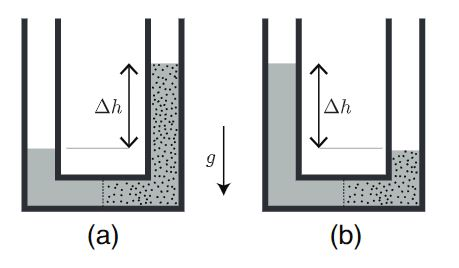
\includegraphics[height=4cm, width=14cm]{1.JPG}
    \end{center}
    \begin{enumerate}
      \item Use the information provided to determine the values of $\Delta H$ and $\Delta G$ for this reaction, for
      one mole of ethanol. Assume that the reaction takes place at $298 K$ and $1$ bar.

        \textcolor{hwColor}{
          \\
          From page 34 of the textbook we have $\Delta H=\Delta U+P ~ \Delta V$, $\Delta H=\Delta Q+\Delta G$, and $\Delta H=H_f-H_i$.
          \\
          \\
          $
            \begin{cases}
              H_f=3 H_2O+2CO_2=3 \bigg( -285.83 \bigg)+2 \bigg( -393.51 \bigg)=-1644.49
              \\
              \\
              H_i=C_2 H_5 OH+3O_2=-277.69+3 \bigg( 0 \bigg)=-277.69
            \end{cases}
            \\
            \\
            \\
            \therefore ~~~ \boxed{\Delta H=-1644.49-\bigg( -277.69 \bigg)=-1366.8 ~ kJ} ~~~~ \checkmark
            \\
            \\
            \\
            \\
            \Delta G=\left[
              \bigg( 3 \bigg( -237.13 \bigg)+2 \bigg( -394.36 \bigg) \bigg)
              -
              \bigg( -174.78+3 \bigg( 0 \bigg) \bigg)
            \right]
            \\
            \\
            \\
            \therefore ~~~ \boxed{\Delta G=-1500.11-\bigg( -174.78 \bigg)=-1325.33 ~ kJ} ~~~~ \checkmark
            \\
            \\
          $
        }

      \item Assuming ideal performance, how much electrical work can you get out of the cell for each
      mole of ethanol fuel?

        \textcolor{hwColor}{
          \\
          The total decrease in Gibbs free energy is converted to electrical energy. Now by knowing $\Delta G$
          the electrical work we can get out of the cell for each mole of ethanol fuel is:
          \\
          \\
          $
            W_e=\Delta G=-1325.33 ~ kJ
            \\
          $
        }

      \item How much waste heat (in kJ) is produced for each mole of ethanol fuel?

        \textcolor{hwColor}{
          \\
          $
            \Delta H=\Delta Q+\Delta G \Longrightarrow Q_{waste}=\Delta H-\Delta G
            =-1366.8 ~ kJ+1325.33 ~ kJ
            \\
            \\
            \\
            \therefore ~~~ \boxed{
              Q_{waste}=-41.47 ~ kJ
            } ~~~~ \checkmark
            \\
            \\
          $
        }

      \item Determine the voltage of the cell if the steps of this reaction are:
      $$
        \text{Reduction at the (-) electrode}: ~ C_2 H_5 OH + 3 H_2 O \longrightarrow 2 CO_2 + 12H^+ + 12e^-
      $$
      $$
        \text{Oxidation at the (+) electrode}: ~ 3O_2 + 12H^+ +12 e^- \longrightarrow 6H_2 O
      $$

        \textcolor{hwColor}{
          \\
          In the previous section we found that $W_e=\Delta G=-1325.33 ~ kJ$. (Followed the steps on page 155 of the textbook)
          $
            V_E=\dfrac{\text{Electrical work done}}{total charge}=\dfrac{|-1325.33 ~ kJ|}{2 \times 6.02 \times 10^{23}}
            \\
            \\
            \therefore ~~~ \boxed{V_E=6.8 ~ eV} ~~~~ \checkmark
            \\
            \\
          $
          By knowing how many electrons are being pushed around the circuit for each molecule. For this case there is 2.
          \\
          \\
        }

    \end{enumerate}

    \item The thermodynamic identity for $G$ is:
    $$
      dG \doteq -S dT+V dP+\mu dN.
    $$
    Use the chain rule to derive partial-derivative expressions for $S, V$ and $\mu$.

      \textcolor{hwColor}{
        \\
        Chapter $5$, pages $156$ and $162$ gwe have. 
        \\
        \\
        $
          \begin{cases}
            dU=TdS-P dV+\mu dN
            \\
            \\
            G \equiv U+PV-TS
          \end{cases}
          \\
          \\
          \\
          dG=dU+d \bigg( PV \bigg)-d \bigg( TS \bigg)
          =dU+dP ~ V+p ~ dV-dT ~ S-T ~ dS
          \\
          \\
          \\
          =\bigg( TdS-P dV+\mu dN \bigg)+dP ~ V+p ~ dV-dT ~ S-T ~ dS
          \\
          \\
          \\
          \therefore ~~~ \boxed{
            \begin{cases}
              \dfrac{\partial G}{\partial P}=V
              \\
              \\
              \dfrac{\partial G}{\partial T}=-S
              \\
              \\
              \dfrac{\partial G}{\partial N}=\mu
            \end{cases}
          } ~~~~ \checkmark
        $
      }

  \end{enumerate}

\end{document}
